\chapter{Introduzione}

I dischi circum-stellari sono delle strutture sottili costituite da gas e polveri che orbitano attorno ad una stella giovane e costituiscono una componente fondamentale del processo di formazione stellare. 
In primo luogo è attraverso il disco che il corpo centrale accresce gran parte della sua massa: questo avviene per mezzo di processi che determinano la ridistribuzione di momento angolare all'interno della struttura orbitante, consentendo al materiale che la costituisce di fluire verso l'interno.
Un secondo ruolo importante svolto dai dischi circumstellari è che sono il luogo dove avviene la formazione planetaria grazie all'aggregazione dei planetesimi: per tale motivo sono detti \textit{proto-planetari}.

La dinamica dei dischi d'accrescimento è fortemente influenzata dalla presenza di corpi perturbanti. In Figura \ref{fig:im_int} è riportata un'immagine nel continuo di dischi d'accrescimento osservati grazie ad ALMA (Atacama Large Millimeter/submillimeter Array).
\begin{figure}[H]
    \centering
    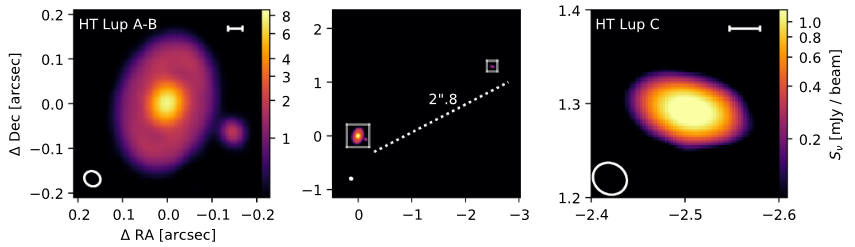
\includegraphics[width=\textwidth]{Immagini/IntroTeorica/immagine_introduzione.png}
    \caption{Immagine nel continuo del sistema HT Lup. La figura centrale mostra la separazione spaziale fra i tre dischi, mentre quella di sinistra evidenzia la struttura dei dischi HT Lup A-B. L'immagine di destra è dedicata a HT Lup C. L'origine del sistema di coordinate è posto nel picco di flusso del disco A \parencite{OsservazioniALMA}. }
    \label{fig:im_int}
\end{figure}
In un sistema binario, ossia formato da due stelle che interagiscono gravitazionalmente fra loro, è possibile osservare tre diversi dischi d'accrescimento: due circum-stellari ed uno circum-binario.
Determinare l'estensione spaziale di un disco proto-planetario in un sistema multiplo è una problematica che richiede lo studio dell'interazione fra un corpo perturbante ed un anello di gas.
Approcci semi-analitici come quello di \textcite{PapaloizouPringle1977}, focalizzato sull'analisi delle forze di marea causate dalla presenza del compagno, e quello di \textcite{GoldreichTremaine1980}, basato sulle risonanze fra le orbite del disco e della binaria, hanno consentito di determinare che la posizione in cui avviene il troncamento dipende dall'eccentricità $e$ del sistema binario, dal mass-ratio $q$, dal parametro adimensionale $\alpha$ che regola la viscosità del materiale orbitante e dalla temperatura $T$ del disco. 
Una metodologia alternativa per lo studio del troncamento è quella delle \textit{test particles} \parencite{Pichardo2005}: il loro approccio è focalizzato su effetti puramente dinamici e non consente di studiare i fenomeni di natura viscosa che regolano l'evoluzione del disco.
Una trattazione più rigorosa del troncamento consiste nel considerare tutta la fisica del problema mediante simulazioni numeriche dell'evoluzione del disco \parencite{ArtymowiczLubow1994}: a causa dell'elevato costo computazionale una vasta regione dello spazio dei parametri resta ad oggi inesplorata.
Questo lavoro di tesi si propone di colmare alcune delle lacune presenti studiando il fenomeno del troncamento nei dischi circumstellari facenti parte di un sistema binario in dipendenza di $\alpha$, $e$ e $q$. 




\section{Struttura della tesi}

La tesi è organizzata nei seguenti 7 capitoli:

\begin{enumerate}
  \item In questo capitolo abbiamo introdotto il problema fisico che vogliamo trattare ed il contesto in cui si presenta. 
  \item Nel Capitolo 2 forniamo un riepilogo della fisica dei dischi proto-planetari, concentrandoci sulla modellizzazione del sistema fisico e sull'evoluzione del disco nel tempo.
  \item Nel Capitolo 3 analizziamo la casistica dei dischi ospitati in sistemi binari. \'E presente un breve riepilogo sul problema di Keplero e sono riportati i diversi approcci presenti in letteratura riguardanti il problema del troncamento.
  \item Nel Capitolo 4 vengono presentati i metodi numerici utilizzati in questo lavoro di tesi. L'esposizione è incentrata su FARGO3D, codice euleriano a griglia sviluppato per lo studio computazionale della fisica dei dischi d'accrescimento.
  \item Il Capitolo 5 è incentrato sulle simulazioni che abbiamo effettuato in questo lavoro di tesi: spieghiamo quale sia il setup simulativo e quali condizioni abbiamo deciso di imporre. Una sezione è dedicata all'esposizione di tutte le tecniche numeriche necessarie per l'analisi dei dati prodotti mediante FARGO3D.
  \item Nel Capitolo 6 sono riportati i risultati ottenuti. La prima sezione riguarda le dimensioni dei dischi, mentre la seconda le eccentricità degli stessi. Nella parte finale del capitolo effettuiamo un confronto con il modello teorico proposto da \textcite{ManaraTronc2019}.
  \item Nel Capitolo 7 riassumiamo i risultati ottenuti e discutiamo i limiti ed i possibili sviluppi futuri di questo lavoro.  
\end{enumerate}